\section{Experiments}

We conduct experiments to answer the following research questions:\\
 
\noindent\mygraybox{%
{\renewcommand{\labelenumi}{\textbf{RQ\arabic{enumi}:}}
\begin{enumerate}
\item \textbf{(Utility):} How much does root-only noising with dependency-aware budget allocation reduce target-node error compared to independent per-release noising?
\item \textbf{(Reconstruction):} Under a MAP adversary with repeated queries at matched per-root noise, how much does $\mathcal{M}$-All's privacy degrade compared to \sysname{}?
\item \textbf{(Structural Analysis):} What structural properties of the template and budget allocation determine when dependency-aware noising provides the largest advantage?
\item \textbf{(Deployment):} Do the mechanism-level findings transfer to a real LLM-driven tool-call deployment?
\end{enumerate}}%
}\\

\noindent\textbf{Summary of Findings.}
\textbf{RQ1:} \sysname{} achieves $2.6\times$ lower aggregate wMAPE than $\mathcal{M}$-All at $\varepsilon = 0.1$ (7.8\% vs.\ 20.3\%, Exponential, $B = (2k{+}1)\varepsilon$), widening to $3.8\times$ at $(3k{+}1)\varepsilon$ and at stronger privacy. Additional adversarial turns improve \sysname{}'s utility while $\mathcal{M}$-All's stays flat.

\textbf{RQ2:} $\mathcal{M}$-All's reconstruction wMAPE drops from $10.2\%$ to $3.2\%$ as $q$ increases from $1$ to $16$ ($\varepsilon_r = 0.1$, Strategy B, informed prior); \sysname{} is invariant. Each adversarial query produces an independent observation that tightens the MAP posterior; \sysname{}'s cached responses contribute no new information after the first release.

\textbf{RQ3:} \sysname{} wins on every template at every budget; the magnitude of the win tracks whether the target formula compresses or amplifies root noise. Compressive templates (AIP, HOMA, FIB4) yield the largest gains ($5.1\times$, $3.9\times$, $4.4\times$ at $B=(3k{+}1)\varepsilon$); amplifying templates (ANEMIA, CONICITY) yield smaller multiplicative gains on already-low absolute errors. The allocation follows $\varepsilon_i \propto (|h_i| D_i)^{1/2}$ (fitted slope 0.50), is mechanism-independent, and reclaims budget from zero-sensitivity roots.

\textbf{RQ4:} The RQ1--3 ordering and per-template structure transfer cell-for-cell to a real LLM-driven deployment (GPT-5.4 nano agent harness, 21{,}600 sessions, 0\% session-level compliance failures), confirming that the privacy-utility tradeoff established at the mechanism level holds end-to-end.
 
% \noindent\textbf{Summary of Findings.} Utility is measured via wMAPE and Risk Class Error; reconstruction vulnerability via a MAP adversary with uniform and informed priors at $q \in \{1, 4, 8\}$ repeated queries (Sec.~\ref{sec:metrics}).
 
% \textbf{RQ1:} \sysname{} achieves $2.3\times$ lower aggregate wMAPE than $\mathcal{M}$-All at $\varepsilon = 0.1$ (7.6\% vs.\ 17.1\%, Exponential, $B = (2k{+}1)\varepsilon$), widening at stronger privacy. A double asymmetry emerges: additional adversarial turns improve \sysname{}'s utility while $\mathcal{M}$-All's stays flat. The win rate increases from 27\% to 65\% as budget grows.
 
% \textbf{RQ2:} $\mathcal{M}$-All's reconstruction wMAPE drops from 6.3\% to 3.2\% as $q$ increases from 1 to 8 ($\varepsilon_r = 0.1$, informed prior); \sysname{} is invariant. Two effects compromise $\mathcal{M}$-All: the target release leaks a cross-root constraint at $q = 1$, and repeated queries enable noise averaging as $q$ grows.
 
% \textbf{RQ3:} The advantage is governed by whether the target formula compresses or amplifies root noise: compressive templates yield large gains (FIB4: $5.1\times$, HOMA: $4.7\times$); amplifying templates yield small losses (ANEMIA: $-0.3$pp). The allocation follows $\varepsilon_i \propto (|h_i| D_i)^{1/2}$ (fitted slope 0.50), is mechanism-independent, and reclaims budget from zero-sensitivity roots.


\subsection{Setup}
\label{sec:exp-setup}
\paragraph{Data.} We use CDC's publicly available National Health and Nutrition
Examination Survey (NHANES) 2017--2018~\cite{nhanes2017exam}, which covers   body measures, blood pressure, hematology, cholesterol, triglycerides, glucose, insulin etc. We consider $8$ clinical templates for diagnosis. Each template defines $k$ root attributes (a subset of the NHANES medical measurements) and a deterministic target function $T$ that computes a clinical index used for diagnosis. For example, the FIB4 template uses four roots (age, AST, PLT, ALT) and computes $T = \text{age} \cdot \text{AST} / (\text{PLT} \cdot \sqrt{\text{ALT}})$. We draw $200$ adult male patients per template from the NHANES population (the per-template subpopulation ranges from $n = 1{,}195$ to $2{,}840$) for RQ1--RQ3, and the first $100$ of these for the deployment evaluation in RQ4. All template details are in App.~\ref{app:med-profiles}.

\paragraph{Interaction model.} Following the threat model (Sec.~\ref{sec:threat-model}), we evaluate a multi-turn interaction over $t \in \{k{+}1,\; 2k{+}1,\; 3k{+}1\}$ turns. In each of the first $t-1$ turns, the adversary requests a root or an arbitrary function of roots; in the final turn, it requests the roots required to compute the target and applies $T$ on the sanitized values it receives. With $k \in \{2, 3, 4\}$, $t$ ranges from 3 to 13, giving $1$, $2$, or $3$ adversarial queries per root. For RQ1--RQ3, we simulate this interaction directly through mechanism implementations to isolate the privacy-utility tradeoff from NER errors and prompt formatting artifacts; RQ4 (Sec.~\ref{sec:experiments-rq4}) re-runs the same threat model end-to-end through an LLM tool-call pipeline.

\paragraph{Mechanisms and configurations.} We evaluate three noise mechanisms (Discrete Exponential~\cite{mcsherry2007mechanism}, Bounded Laplace, Staircase~\cite{geng2015optimal}) under the three configurations of Sec.~\ref{sec:exploiting-dependencies} ($\mathcal{M}$-All, $\mathcal{M}$-Roots, $\mathcal{M}$-Opt). All operate in normalized index space with $m = 1{,}000$ candidates. Table~\ref{tab:baseline_summary} summarizes the configurations; mechanism details are in App.~\ref{app:baselines}.

% \paragraph{Mechanisms and configurations.} We evaluate three noise mechanisms (Discrete Exponential~\cite{mcsherry2007mechanism}, Bounded Laplace, Staircase~\cite{geng2015optimal}) under three configurations ($\mathcal{M}$-All, $\mathcal{M}$-Roots, $\mathcal{M}$-Opt) defined in Sec.~\ref{sec:method}. All operate in normalized index space with $m = 1{,}000$ candidates and total budget $B = t \cdot \varepsilon$. Table~\ref{tab:baseline_summary} summarizes the configurations. Mechanism details are in App.~\ref{app:baselines}.

\paragraph{Budgets and allocation.} All methods share total budget $B = t \cdot \varepsilon$. RQ1 sweeps 10 privacy levels $\varepsilon \in [0.005, 5.0]$ across three adversary turn budgets $t \in \{k{+}1, 2k{+}1, 3k{+}1\}$; RQ2 fixes per-root noise $\varepsilon_r \in \{0.05, 0.1, 0.5, 1.0\}$ and varies adversarial queries $q \in \{1, 4, 8, 16\}$. The three configurations distribute $B$ differently: $\mathcal{M}$-All assigns $\varepsilon$ to each of the $t$ releases; $\mathcal{M}$-Roots distributes $B$ uniformly across $k$ roots ($\varepsilon_i = t\varepsilon/k$); $\mathcal{M}$-Opt allocates per the sensitivity-weighted solution of Sec.~\ref{sec:opt-budget} ($\varepsilon_i \propto \sqrt{|h_i| \cdot \delta_i}$). Roots saturating at $\varepsilon_{\min}$ have their budget redistributed to active roots.

\paragraph{Domain knowledge.} \sysname{} uses two forms of public knowledge, neither dependent on the private patient data: \textit{domain bounds} $[\ell_i, u_i]$ from the per-template NHANES adult male subpopulation, and \textit{population-mean root values} $\mu$ from the same population (excluding test samples) for evaluating sensitivities $h_i = |\partial T / \partial x_i(\mu)|$. The $B$-mDP guarantee holds regardless, as domain knowledge affects only utility.

\paragraph{Text-DP reference.} We additionally include CAPE-F~\cite{wu2025capecontextawarepromptperturbation} as a text-DP reference, adapted to numeric values by constraining decoding to numerical characters. CAPE-F operates under a different DP definition and is not directly comparable on $\varepsilon$; we include it to demonstrate that text-based DP is fundamentally unsuitable for structured numeric data.

% \subsubsection{\textbf{Interaction Model}}
% \label{sec:interaction-model}
 
% Following the threat model of Sec.~\ref{sec:threat-model}, we evaluate a multi-turn interaction between the user agent $\mathcal{U}$ and the adversary $\mathcal{A}$. In each turn except the last, $\mathcal{A}$ may request an arbitrary function of the user's root values. In the final turn, $\mathcal{A}$ forces the user to compute the target value $T$ and returns the diagnosis. The adversary's turn budget determines how many times it can probe each root before the task must be completed.
 
% We parameterize the number of turns as $t \in \{k{+}1,\; 2k{+}1,\; 3k{+}1\}$, where $k$ is the number of roots for the template. This gives the adversary $1$, $2$, or $3$ queries per root (plus one turn for the target), representing increasing adversary strength. Since $k$ varies across templates ($k \in \{2, 3, 4\}$), $t$ ranges from $3$ to $13$.
 
% Under $\mathcal{M}$-All, each request is answered by computing the requested value from the original (unsanitized) roots and applying fresh, independent noise. Under \sysname{}, roots are noised once at the start of the interaction; all subsequent requests are answered deterministically from the cached noised roots.
 
% This parameterization produces a double asymmetry:
% \begin{itemize}
%     \item \textbf{Utility.} More turns increase the total budget $B = t \cdot \varepsilon$, giving \sysname{} more per-root budget and better target utility. $\mathcal{M}$-All's target utility is unaffected --- the target is a single independent release at parameter $\varepsilon$ regardless of $t$.
%     \item \textbf{Privacy.} More turns give the adversary more independent observations under $\mathcal{M}$-All, degrading privacy. Under \sysname{}, all queries are post-processing and carry no new information.
% \end{itemize}
 
% \noindent Additional adversarial turns simultaneously \emph{help} \sysname{} (more budget) and \emph{hurt} $\mathcal{M}$-All (more leakage).
 
% \paragraph{Simulation.} We simulate the worst-case adversary by directly computing and sanitizing values through the mechanism implementations, bypassing the natural language pipeline. This isolates the privacy-utility tradeoff from NER errors, LLM variability, and prompt formatting artifacts. Root values are drawn from NHANES, sanitized by the mechanism under test, and target values are computed from the noised or true roots according to the template formulas.


% \paragraph{Total Privacy Budget}
%  All methods are constrained to the same total budget $B = t \cdot \varepsilon$, where $\varepsilon$ is the per-release budget and $t$ is the number of turns. The three configurations (Sec.~\ref{sec:baselines}) differ in how this budget is distributed:
% \begin{itemize}
%     \item $\mathcal{M}$-All: each of the $t$ releases receives $\varepsilon$.
%     \item $\mathcal{M}$-Roots: the budget $B = t\varepsilon$ is distributed uniformly across $k$ roots, giving each root $\varepsilon_i = t\varepsilon / k$.
%     \item $\mathcal{M}$-Opt: the budget $B = t\varepsilon$ is distributed across roots according to the sensitivity-weighted allocation (Sec.~\ref{sec:opt-budget}).
% \end{itemize}

% \subsubsection{\textbf{Domain Knowledge}}
% \label{sec:domain-knowledge}
% \sysname{} exploits two forms of public domain knowledge, neither of which depends on the private patient data being sanitized.
 
% \begin{itemize}
%     \item \textbf{Domain bounds} $[\ell_i, u_i]$ for each root are set to the observed min--max of the per-template NHANES adult male subpopulation. These bounds define the grid spacing $\delta_i = D_i/(m{-}1)$ and the support of all three noise mechanisms.
%     \item \textbf{Population-mean root values} $\mu = (\mu_1, \dots, \mu_k)$ are computed from the same NHANES reference population, excluding the test samples used for evaluation. These means serve as the operating point at which target sensitivities $h_i = |\partial T / \partial x_i(\mu)|$ are evaluated for budget allocation (Sec.~\ref{sec:opt-budget}).
% \end{itemize}
 
% \noindent Both quantities are properties of the reference population, not of any individual patient. The privacy guarantee of $B$-mDP holds regardless of the domain knowledge used as it affects only the utility of the allocation.

% We evaluate three noise mechanisms---Discrete Exponential, Bounded Laplace, and Staircase---each in three progressive configurations that isolate the contributions of our two structural optimizations. All three mechanisms operate under the same privacy definition ($\varepsilon$-mDP), the same total budget ($B = t \cdot \varepsilon$), and the same discretization ($m = 1{,}000$ candidates per domain). The key differences lie in the noise distribution and in \emph{how} each configuration distributes its budget and \emph{which values} it noises. Table~\ref{tab:baseline_summary} summarizes these variants.
 
% \subsubsection{\textbf{Shared setup: index-space operation.}}
% \label{sec:index-space}
% All three mechanisms operate in normalized index space. Given a true value $x_i \in [\ell_i, u_i]$ with domain width $D_i = u_i - \ell_i$ and grid spacing $\delta_i = D_i/(m{-}1)$, the value is mapped to an index $t_i = (x_i - \ell_i)/\delta_i \in [0, m{-}1]$. The mechanism produces a noisy index $s$, and the output is $x'_i = s\,\delta_i + \ell_i$. The sensitivity in index space is 1 for all three mechanisms.
 
% \subsubsection{\textbf{Privacy Mechanisms.}}
% \label{sec:baselines}
 
% \paragraph{Discrete Exponential (Exp).}
% The mechanism samples index $s$ with probability $P(s) \propto \exp(-\varepsilon_i\,|t_i - s|/2)$. This is the standard exponential mechanism~\cite{mcsherry2007mechanism} with utility function $u(s) = -|t_i - s|$ and sensitivity $\Delta u = 1$.
 
% \paragraph{Bounded Laplace (BLap).}
% The mechanism draws continuous noise $Z \sim \mathrm{Lap}(0, 1/\varepsilon_i)$ in index space, clamps the noisy index to $[0, m{-}1]$, and rounds to the nearest integer. The Laplace distribution on $\mathbb{R}$ satisfies $\varepsilon_i$-mDP; clamping and rounding are deterministic post-processing and preserve the guarantee. See App.~\ref{app:blap-alloc} for details.
 
% \paragraph{Staircase (Stair).}
% The mechanism~\cite{geng2015optimal} draws noise from the Geng--Viswanath staircase distribution with sensitivity 1 and parameter $\varepsilon_i$, then clamps and rounds as in BLap. The staircase distribution replaces the Laplace's smooth density with a piecewise-constant density that is optimal for single-query pure $\varepsilon$-DP. See App.~\ref{app:stair-alloc} for details.
 
% \subsubsection{\textbf{Configurations}}
% Each mechanism is evaluated in three configurations that progressively add structural knowledge (corresponding to the levels defined in Sec.~\ref{sec:exploiting-dependencies}):
 
% \paragraph{$\mathcal{M}$-All (independent noising, baseline).}
% Each request from the adversary is answered by computing the requested value from the original (unsanitized) root values and applying fresh, independent noise at parameter $\varepsilon$. No knowledge of the DAG structure is used --- each release is treated as an independent value to protect. This is equivalent to vanilla Preempt~\cite{chowdhury2025} for the Exponential mechanism, and serves as the ``no structural knowledge'' reference for all three mechanisms.
 
% \paragraph{$\mathcal{M}$-Roots (root-only + uniform allocation).}
% Only the $k$ root nodes are noised; all requests are answered deterministically from the cached noised roots via post-processing (Sec.~\ref{sec:method}). The total budget $B = t \cdot \varepsilon$ is distributed uniformly across roots, giving each root $\varepsilon_i = t\varepsilon/k$. Since $t > k$, each root receives more budget than under $\mathcal{M}$-All. This creates a clean ablation: the improvement from $\mathcal{M}$-All to $\mathcal{M}$-Roots isolates the gain from \emph{eliminating redundant noising and concentrating budget on roots}.
 
% \paragraph{$\mathcal{M}$-Opt (root-only + sensitivity-based allocation).}
% As in $\mathcal{M}$-Roots, only root nodes are noised and all requests are post-processed. The total budget $B = t \cdot \varepsilon$ is distributed across roots according to the sensitivity-weighted allocation $\varepsilon_i \propto \sqrt{|h_i| \cdot \delta_i}$ (Sec.~\ref{sec:opt-budget}), where $h_i = |\partial T / \partial x_i(\mu)|$ is the population-mean sensitivity. The improvement from $\mathcal{M}$-Roots to $\mathcal{M}$-Opt isolates the gain from \emph{dependency-aware budget allocation}.
 
% \subsubsection{\textbf{Text-DP reference.}}
 
% In addition to the nine numeric-DP conditions above, we include \textbf{CAPE-F}~\cite{wu2025capecontextawarepromptperturbation} as a text-DP reference point. CAPE-F is a context-aware perturbation mechanism that combines MLM logits with embedding distances to select replacement tokens, adapted to numeric values by constraining decoding to numerical characters. CAPE-F operates under a different DP definition and is not directly comparable on $\varepsilon$; it is included to demonstrate that text-based DP mechanisms are fundamentally unsuitable for structured numeric data, regardless of the privacy budget.
 
\begin{table}[h]
\centering
\caption{Summary of experimental conditions. All numeric methods use $\varepsilon$-mDP on the same index-space grid ($m = 1{,}000$) with the same total budget $B = t \cdot \varepsilon$, where $t$ is the number of interaction turns. CAPE-F is a text-DP reference under a different DP definition.}
\label{tab:baseline_summary}
\resizebox{\columnwidth}{!}{%
\begin{tabular}{@{}lccc|c@{}}
\toprule
& \multicolumn{3}{c|}{\textbf{Numeric $\varepsilon$-mDP}} & \textbf{Text-DP} \\
\textbf{Property} & \textbf{$\mathcal{M}$-All} & \textbf{$\mathcal{M}$-Roots} & \textbf{$\mathcal{M}$-Opt (\sysname)} & \textbf{CAPE-F} \\
\midrule
Mechanisms & Exp / BLap / Stair & Exp / BLap / Stair & Exp / BLap / Stair & Bucket Exp. \\
Budget alloc. & Uniform ($\varepsilon$/release) & Uniform ($t\varepsilon/k$/root) & $\propto \sqrt{|h_i| \cdot \delta_i}$ & Per-token \\
Values noised & Each release & Roots only ($k$) & Roots only ($k$) & All \\
Post-processing & \ding{55} & \ding{51} & \ding{51} & \ding{55} \\
DAG-aware & \ding{55} & \ding{55} & \ding{51} & \ding{55} \\
Ext.\ models & None & None & None & RoBERTa \\
DP guarantee & $\varepsilon$-mDP & $\varepsilon$-mDP & $\varepsilon$-mDP & $(\varepsilon{+}\varepsilon')$-DP \\
\bottomrule
\end{tabular}%
}
\end{table}

\subsection{Metrics}
\label{sec:metrics}
We evaluate each sanitization method along two axes: \emph{numeric accuracy} of the target clinical index, and \emph{clinical decision preservation}. Both are measured at the target node of each template---the final derived value from which the clinical risk class is determined. Let $y$ denote the ground truth target value and $\hat{y}$ the target value obtained from (possibly noised) inputs.

\paragraph{Weighted Mean Absolute Percentage Error (wMAPE)}
For each template with $N$ samples, we compute:
\begin{equation}
\text{wMAPE} = \frac{\sum_{i=1}^{N} |\hat{y}_i - y_i|}{\sum_{i=1}^{N} |y_i|} \times 100\%
\end{equation}
the mean absolute error normalized by the mean ground-truth magnitude~\cite{hyndman2006another,kolassa2007advantages}. A wMAPE of 0\% indicates perfect numeric preservation; values above 100\% indicate that average distortion exceeds the typical value of the index. We use wMAPE rather than per-sample MAPE because MAPE is unstable when ground-truth values approach zero (e.g., FIB4 typical value ${\sim}1$ within $[0.12, 37.95]$; AIP typical value ${\sim}0.4$ within $[-0.64, 1.97]$).


\paragraph{Risk Class Error.}
Each template defines clinically meaningful risk categories based on published threshold values (App.~\ref{app:med-profiles}). For example, the FIB-4 template classifies patients into Low ($< 1.30$), Indeterminate ($1.30$--$2.67$), or High ($> 2.67$) fibrosis risk. We map both the ground truth and sanitized target values to their respective risk classes $c(y)$ and $c(\hat{y})$, then compute:
\begin{equation}
\text{Risk Class Error} = \frac{1}{N} \sum_{i=1}^{N} \frac{|c(\hat{y}_i) - c(y_i)|}{C - 1} \times 100\%
\end{equation}
where $C$ is the number of risk classes for the profile ($C = 3$ for ANEMIA, AIP, FIB4, HOMA; $C = 2$ for the remaining profiles). This metric directly measures \emph{clinical harm}: a Risk Class Error of 0\% means that sanitization never changes the clinical decision, regardless of numeric distortion. The two metrics are complementary: a method may achieve low wMAPE but non-zero RCE if perturbations cross decision boundaries.

% \noindent The two metrics capture complementary aspects of utility. A method can achieve low wMAPE (small numeric perturbation) while still incurring non-zero Risk Class Error if the perturbation crosses a decision boundary. Conversely, a method with higher wMAPE may preserve risk classes perfectly if the noise stays within the same classification band. \sysname{}'s budget allocation is formulated to minimize absolute error at the target, but the resulting improvement in numeric accuracy typically translates to improved risk class preservation as well.






\subsection{RQ1: Target Utility Under Adversarial Queries}
\label{sec:experiments-rq1}


\providecommand{\pmstd}[1]{{\scriptsize $\pm$#1}}

\begin{table*}[t]
\centering
\setlength{\tabcolsep}{2.8pt}
\small
\caption{Aggregate wMAPE (\%) at mid-to-high privacy levels across three adversary budget levels (Exponential mechanism). $\bar{B}$: average total budget across templates. $\mathcal{M}$-All is invariant to the budget level; $\mathcal{M}$-Opt improves with each additional adversarial turn. Aggregate values are the mean across 8 templates; bootstrap SEs are propagated from per-template SEs as $\sqrt{\sum_t \mathrm{SE}_t^2}/k$. At $\varepsilon \geq 1.0$, all methods achieve $\leq 1\%$ wMAPE and differences are negligible (see App.~\ref{app:rq1-tables}).}
\label{tab:double_asymmetry}
\begin{tabular}{c|cccc|cccc|cccc}
\toprule
& \multicolumn{4}{c|}{$B = (k{+}1)\varepsilon$} & \multicolumn{4}{c|}{$B = (2k{+}1)\varepsilon$} & \multicolumn{4}{c}{$B = (3k{+}1)\varepsilon$} \\
$\varepsilon$ & $\bar{B}$ & All & Roots & Opt & $\bar{B}$ & All & Roots & Opt & $\bar{B}$ & All & Roots & Opt \\
\midrule
0.5 & 1.81 & 5.6\pmstd{0.30} & 4.0\pmstd{0.25} & \textbf{2.7\pmstd{0.13}} & 3.12 & 5.7\pmstd{0.30} & 2.4\pmstd{0.13} & \textbf{1.7\pmstd{0.09}} & 4.44 & 5.9\pmstd{0.33} & 1.8\pmstd{0.10} & \textbf{1.2\pmstd{0.05}} \\
0.2 & 0.73 & 12.6\pmstd{0.64} & 10.1\pmstd{0.47} & \textbf{6.6\pmstd{0.29}} & 1.25 & 12.3\pmstd{0.62} & 5.9\pmstd{0.37} & \textbf{4.5\pmstd{0.22}} & 1.78 & 12.2\pmstd{0.55} & 4.6\pmstd{0.29} & \textbf{3.3\pmstd{0.20}} \\
0.1 & 0.36 & 20.5\pmstd{0.88} & 14.9\pmstd{0.67} & \textbf{13.6\pmstd{0.65}} & 0.62 & 20.3\pmstd{0.96} & 11.4\pmstd{0.57} & \textbf{7.8\pmstd{0.32}} & 0.89 & 21.5\pmstd{0.96} & 8.7\pmstd{0.47} & \textbf{5.6\pmstd{0.26}} \\
0.05 & 0.18 & 35.0\pmstd{1.45} & 26.0\pmstd{1.11} & \textbf{21.6\pmstd{0.94}} & 0.31 & 33.8\pmstd{1.69} & 18.0\pmstd{0.80} & \textbf{13.3\pmstd{0.58}} & 0.44 & 33.7\pmstd{1.75} & 14.3\pmstd{0.68} & \textbf{11.2\pmstd{0.57}} \\
0.02 & 0.07 & 70.3\pmstd{4.35} & 55.5\pmstd{6.81} & \textbf{46.0\pmstd{2.80}} & 0.12 & 75.7\pmstd{10.89} & 34.1\pmstd{1.55} & \textbf{29.2\pmstd{1.23}} & 0.18 & 72.3\pmstd{5.10} & 27.9\pmstd{1.29} & \textbf{21.9\pmstd{0.96}} \\
0.01 & 0.04 & 122.5\pmstd{10.10} & 101.9\pmstd{9.58} & \textbf{86.6\pmstd{6.21}} & 0.06 & 112.6\pmstd{8.41} & 63.0\pmstd{5.39} & \textbf{48.3\pmstd{2.62}} & 0.09 & 129.5\pmstd{9.85} & 47.3\pmstd{2.59} & \textbf{37.3\pmstd{1.58}} \\
\bottomrule
\end{tabular}
\end{table*}


We evaluate target-node utility under the adversary budgets defined in Sec.~\ref{sec:exp-setup}. $\mathcal{M}$-All noises each root release independently at $\varepsilon$, computing the target deterministically from the latest noised values at the target turn. $\mathcal{M}$-Roots and $\mathcal{M}$-Opt distribute the full budget $B$ across roots once at initialization, then post-process all subsequent releases.

% We evaluate the target-node utility of \sysname{} under a worst-case adversarial query model. The adversary controls $t$ turns of interaction, forcing the user agent to release a sanitized value in each turn. In the final turn, the adversary forces release of the target clinical index $T = g(x)$.

% \paragraph{\textbf{Methods.}}
% \begin{itemize}
%     \item $\mathcal{M}$-All: sanitizes the target directly with $\varepsilon$ (a single independent draw from the mechanism). The remaining $t-1$ adversarial queries produce independent draws that do not affect target utility.
%     \item $\mathcal{M}$-Roots: noises the $k$ root nodes once with total budget $B$ distributed uniformly ($B/k$ per root). All subsequent queries---including the target---are computed deterministically from the noised roots.
%     \item $\mathcal{M}$-Opt: same as $\mathcal{M}$-Roots but allocates $B$ across roots proportionally to their influence on the target, using dependency-aware budget allocation (Sec.~\ref{sec:baselines}).
% \end{itemize}
% We evaluate each variant under three mechanisms: Exponential (Exp), Bounded Laplace (BLap), and Staircase (Stair), yielding 9 method configurations.

% \paragraph{\textbf{Budget settings.}}
% The total budget consumed by the adversary is $B = t \cdot \varepsilon$. Crucially, $\mathcal{M}$-All uses only $\varepsilon$ for the target release regardless of $B$, while $\mathcal{M}$-Roots and $\mathcal{M}$-Opt can distribute the full $B$ across root nodes. We evaluate three $k$-dependent budget levels representing increasing adversarial strength:

% \begin{table}[h]
% \centering
% \small
% \caption{Budget per template under each adversarial setting ($B / \varepsilon$). $k$: number of root nodes.}
% \label{tab:rq1_budget}
% \begin{tabular}{lcccc}
% \toprule
% \textbf{Template} & $k$ & $k{+}1$ & $2k{+}1$ & $3k{+}1$ \\
% \midrule
% ANEMIA, AIP, CONICITY & 3 & 4 & 7 & 10 \\
% FIB4 & 4 & 5 & 9 & 13 \\
% VASCULAR, TYG, HOMA, NLR & 2 & 3 & 5 & 7 \\
% \bottomrule
% \end{tabular}
% \end{table}

\paragraph{Data.} We use the same 8 clinical templates and 200-patient NHANES 2017--2018 test split as in the experimental setup (Sec.~\ref{sec:exp-setup}), across 10 privacy budgets $\varepsilon \in [0.005, 5.0]$.

% ────────────────────────────────────────────────────────────────────────
% \subsubsection{What governs the magnitude of \sysname{}'s advantage?}
% Under the root-only configurations, the target perturbation depends on how the formula $g$ amplifies or compresses each root's noise (captured by $|h_i| = |\partial g / \partial x_i|$). Templates whose target formulas \emph{compress} root noise (e.g., divisions, products with large constants) yield the largest gaps between $\mathcal{M}$-All and \sysname{} --- root-domain noise gets attenuated en route to the target, while $\mathcal{M}$-All's per-release noise compounds across roots in a Lipschitz-amplified way (Sec.~\ref{sec:nonlinear-amplification}). Templates whose formulas \emph{amplify} root noise into a narrow target domain show smaller absolute errors for both configurations, with \sysname{} retaining a multiplicative advantage on a smaller base. Two structural factors further modulate the gap: (i) \textit{budget concentration} --- each root receives $t/k$ times $\mathcal{M}$-All's per-release budget, so higher $t/k$ favors root-only noising; (ii) \textit{zero-sensitivity roots} --- some roots (e.g., RBC for MCHC, TC for AIP) waste budget under $\mathcal{M}$-Roots; $\mathcal{M}$-Opt clamps them at $\varepsilon_{\min}$ and redistributes the freed budget to active roots.

% ────────────────────────────────────────────────────────────────────────

\subsubsection{Aggregate results.}
Table~\ref{tab:double_asymmetry} reports aggregate wMAPE for the Exponential mechanism. The ordering $\mathcal{M}$-All $>$ $\mathcal{M}$-Roots $>$ $\mathcal{M}$-Opt holds at every $\varepsilon$ and every budget level, confirming that root-only noising and dependency-aware allocation provide additive gains; BLap and Stair follow the same trend (App.~\ref{app:rq1-tables}). At $\varepsilon = 0.1$ and $B = (2k{+}1)\varepsilon$, Exp-Opt achieves 7.8\% vs.\ 20.3\% for Exp-All --- a $2.6\times$ improvement, widening to $3.8\times$ at $(3k{+}1)\varepsilon$ ($5.6\%$ vs.\ $21.5\%$). The gap also widens at lower $\varepsilon$: at $\varepsilon = 0.01$, $B = (2k{+}1)\varepsilon$, the gap is $48.3\%$ vs.\ $112.6\%$.

% \subsubsection{Aggregate results.}
% Table~\ref{tab:double_asymmetry} reports the aggregate wMAPE for the Exponential mechanism across all three budget levels. At $B = (2k{+}1)\varepsilon$ and above, the results demonstrate a consistent ordering: $\mathcal{M}$-All $>$ $\mathcal{M}$-Roots $>$ $\mathcal{M}$-Opt (decreasing error), confirming that both root-only noising and dependency-aware allocation provide additive gains. The Bounded Laplace and Staircase mechanisms follow the same trend; full tables for all three mechanisms and budget levels are in App.~\ref{app:rq1-tables}.
 
% At the minimal budget $B = (k{+}1)\varepsilon$, however, $\mathcal{M}$-Roots can underperform $\mathcal{M}$-All --- the budget concentration of $t/k \approx 1.3$--$1.5$ per root is insufficient to overcome the propagation penalty from noising at the root level. This effect is consistent across all three mechanisms. Notably, $\mathcal{M}$-Opt still outperforms $\mathcal{M}$-All even at this minimal budget, demonstrating that the sensitivity-weighted allocation (Level~3) provides gains that uniform root allocation (Level~1) alone cannot.
 
% At $\varepsilon = 0.1$ and $B = (2k{+}1)\varepsilon$, Exp-Opt achieves 7.6\% aggregate wMAPE compared to 17.1\% for Exp-All---a 2.3$\times$ improvement. The gap widens at lower $\varepsilon$: at $\varepsilon = 0.01$, Exp-Opt achieves 49.0\% vs.\ 166\% for Exp-All.
% ────────────────────────────────────────────────────────────────────────
% \subsubsection{\textbf{Budget scaling: the double asymmetry.}}
% \label{sec:double-asymmetry}

% A key property of the adversarial model is that $\mathcal{M}$-All's target utility depends only on $\varepsilon$, not on $B$---the adversary's additional queries are independent draws that do not affect the final target release. In contrast, $\mathcal{M}$-Roots and $\mathcal{M}$-Opt benefit from every unit of additional budget, since more budget means less noise per root.

% Table~\ref{tab:double_asymmetry} illustrates this \emph{double asymmetry} across six privacy levels. The $\mathcal{M}$-All columns are nearly identical across budget levels --- the target is always a single release at $\varepsilon$. The $\mathcal{M}$-Opt columns decrease left-to-right as additional budget is concentrated on roots. At $\varepsilon = 0.1$, Exp-Opt improves from 13.1\% ($k{+}1$) to 7.6\% ($2k{+}1$) to 5.7\% ($3k{+}1$), while Exp-All stays at ${\sim}17\%$. At $\varepsilon \geq 1.0$, all methods achieve $\leq 1\%$ wMAPE and differences are negligible (see App.~\ref{app:rq1-tables}).

% Table~\ref{tab:rq1_win_rate} quantifies the effect per template: the fraction of (template, $\varepsilon$, mechanism) triples where $\mathcal{M}$-Opt achieves lower wMAPE than $\mathcal{M}$-All increases from 27\% at $B = (k{+}1)\varepsilon$ to 42\% at $(2k{+}1)\varepsilon$ to 65\% at $(3k{+}1)\varepsilon$. FIB4 and HOMA are consistent wins at all budget levels; templates like VASCULAR and CONICITY transition from losses to wins as root budget grows.

\subsubsection{Budget scaling: the double asymmetry.}
\label{sec:double-asymmetry}
 
$\mathcal{M}$-All's target utility depends only on $\varepsilon$, not $B$ --- the target is computed from a single fresh draw per root at the target turn, so the adversary's additional turns do not improve target accuracy. $\mathcal{M}$-Roots and $\mathcal{M}$-Opt benefit from every unit of additional budget. Table~\ref{tab:double_asymmetry} illustrates this \emph{double asymmetry}: $\mathcal{M}$-All columns are nearly flat across budget levels, while $\mathcal{M}$-Opt columns decrease as budget concentrates on roots. At $\varepsilon = 0.1$, Exp-Opt improves from 13.6\% ($k{+}1$) to 7.8\% ($2k{+}1$) to 5.6\% ($3k{+}1$), while Exp-All stays at ${\sim}20$--$21\%$. \sysname{} wins on every (template, mechanism) cell at every budget level (Sec.~\ref{sec:experiments-rq3}); the multiplicative advantage \emph{grows} with $B$, driven by templates with compressive target formulas (FIB4, HOMA, AIP).

% Per-template analysis (Sec.~\ref{sec:experiments-rq3}) shows that the aggregate wins are driven by templates with compressive target formulas (FIB4, HOMA), with the win rate increasing from 27\% at $B = (k{+}1)\varepsilon$ to 65\% at $(3k{+}1)\varepsilon$.

% ────────────────────────────────────────────────────────────────────────
% \subsubsection{\textbf{CAPE-F: text-DP reference.}}
% CAPE-F achieves 263--403\% wMAPE across all privacy levels, $65$--$125\times$ worse than BLap-Opt. Its error is essentially flat across $\varepsilon$---the $1.5\times$ ratio from $\varepsilon = 5.0$ to $\varepsilon = 0.005$ compares to BLap-Opt's $225\times$---confirming that the error is dominated by the linguistic-vs-numeric utility mismatch rather than privacy noise. This is because the embedding model cannot capture the relationship between numerical tokens and the rest of the context. As a result, the sampled values often have no semantic bearing to the actual medical condition of the patient. For example, ``$0$'' might get replaced by ``$00$'', which immediately increases error by an order of magnitude.

% % ────────────────────────────────────────────────────────────────────────
% \paragraph{\textbf{Caveats for comparison.}} Even on templates where $\mathcal{M}$-All achieves lower target wMAPE, both methods produce small absolute errors (ANEMIA: 0.3pp difference; CONICITY: 0.1pp). More importantly, the $t - 1$ adversarial turns that precede the target release have no utility cost for either method --- but they have a severe privacy cost for $\mathcal{M}$-All. Each adversarial query produces an independent noisy observation that a reconstruction adversary can exploit, while \sysname{}'s post-processed responses reveal no additional information. The same budget scaling that improves \sysname{}'s utility simultaneously degrades $\mathcal{M}$-All's privacy. We quantify this asymmetry in Sec.~\ref{sec:experiments-rq2}.


\subsubsection{}{Text-DP reference (CAPE-F).} CAPE-F~\cite{wu2025capecontextawarepromptperturbation}, a text-DP mechanism adapted to numeric tokens, achieves $263$--$403\%$ wMAPE across all $\varepsilon$ ($65$--$125\times$ worse than BLap-Opt) and is essentially flat across the privacy axis, confirming that text-DP is unsuitable for structured numeric data regardless of $\varepsilon$.

% \subsubsection{CAPE-F: text-DP reference.}
% It achieves $263$--$403$\% wMAPE across all $\varepsilon$, $65$--$125\times$ worse than BLap-Opt. Its error is essentially flat across $\varepsilon$ (the $1.5\times$ ratio from $\varepsilon = 5.0$ to $0.005$ compares to BLap-Opt's $225\times$), confirming the error is dominated by linguistic-vs-numeric mismatch rather than privacy noise. The embedding model cannot capture relationships between numerical tokens and context: ``$0$'' might be replaced by ``$00$'', immediately increasing error by an order of magnitude.
 
\paragraph{Privacy cost of extra turns.} The $t-1$ adversarial turns preceding the target have no utility cost for either method, but they impose a severe privacy cost on $\mathcal{M}$-All --- each query produces an independent observation a reconstruction adversary can exploit, while \sysname{}'s post-processed responses reveal no additional information. We quantify this in Sec.~\ref{sec:experiments-rq2}.

\paragraph{Privacy cost of extra turns.} The $t-1$ adversarial turns preceding the target have no utility cost for either method, but they impose a severe privacy cost on $\mathcal{M}$-All --- each query produces an independent observation a reconstruction adversary can exploit, while \sysname{}'s post-processed responses reveal no additional information. We quantify this in Sec.~\ref{sec:experiments-rq2}.


% \paragraph{Why not concentrate $\mathcal{M}$-All's budget on the target?}
% A natural alternative is to give $\mathcal{M}$-All the full $B = t\varepsilon$ on the target release, ignoring the $t-1$ adversarial turns. Our threat model rules this out: the adversary controls the interaction, and the user does not know in advance which release will be the target. A user that allocates $B$ to a single release exposes itself to an adversary that simply asks for that release first and exits, leaving $\mathcal{M}$-All with no budget left for legitimate queries. Equivalently, in any strategy that allocates a budget across $t$ unknown future requests, $\mathcal{M}$-All must spend per-release; \sysname{} avoids this dilemma by treating all releases as post-processing of the initial root noising, so allocation is decoupled from request order. Across the $t$ release sequence we evaluate, $\mathcal{M}$-All's per-release budget $\varepsilon$ is the unique strategy that yields the same $\varepsilon$-mDP guarantee on every individual release.


\subsection{RQ2: Reconstruction Attacks}
\label{sec:experiments-rq2}

RQ1 showed $\mathcal{M}$-All's adversarial turns yield no utility benefit. We now ask: do they impose a \emph{privacy cost}? The accumulation analysis (Sec.~\ref{sec:redundancy-noising}) predicts that each independent release gives the adversary a fresh observation, enabling MAP reconstruction that improves with query count. We test this by varying the number of queries under matched per-root noise.

% RQ1 showed that $\mathcal{M}$-All's adversarial turns have no utility benefit --- the target is a single independent release at $\varepsilon$. We now ask: do these turns have a \emph{privacy cost}? The accumulation analysis (Sec.~\ref{sec:redundancy-noising}) predicts that each independent release gives the adversary a fresh observation, enabling MAP reconstruction that improves with query count. We test this prediction by comparing reconstruction under matched per-root noise, varying the number of queries.

\subsubsection{Setup.}
We fix per-root noise $\varepsilon_r \in \{0.05, 0.1, 0.5, 1.0\}$ and vary the adversarial query count $q \in \{1, 4, 8, 16\}$. $\mathcal{M}$-All produces a fresh independent draw per query; $\mathcal{M}$-Roots noises each root once at $\varepsilon_r$ and caches; $\mathcal{M}$-Opt noises each root once under the sensitivity-weighted allocation of total budget $B = k\varepsilon_r$. Method-agnostic RNG seeding makes $\mathcal{M}$-All's first draw and the $\mathcal{M}$-Roots cached value bit-identical at any $(\text{template}, \text{root}, \text{sample})$ triple, so any $q \geq 1$ difference is purely independent-draws vs.\ caching.

\paragraph{Adversary strategies.} \emph{Strategy A (single-root, worst-case):} the adversary concentrates all $q$ queries on $r^* = \arg\max_r \varepsilon_r^{\mathrm{Opt}}$ --- the root with the least noise under $\mathcal{M}$-Opt and therefore the most reconstructable. The target turn additionally forces release of $r^*$, so the adversary observes $q{+}1$ values on $r^*$: under $\mathcal{M}$-All, $q{+}1$ fresh independent draws; under cached methods, $q{+}1$ identical replays. We report MAE on the targeted root only. \emph{Strategy B (all-roots, average-case):} the adversary distributes $q$ queries per root across all $k$ roots, with one extra observation per root from the target turn. We report mean MAE across roots.

\paragraph{MAP adversary and priors.} The adversary performs a per-root 1-D argmax with full knowledge of the sanitization pipeline: $\hat{x}_r = \arg\max_x \prod_i p_{\mathcal{M}}(\tilde{y}_i \mid x, \varepsilon_r) \cdot \pi(x)$. The factorization across roots is exact: under both $\mathcal{M}$-All and the cached methods, per-root observations are independent given the true value, and the user agent never releases a value that couples roots through the target. Unobserved roots return the prior mean (Strategy A only). For cached methods, the per-root likelihood collapses to a single factor regardless of $q$. We evaluate two priors --- \emph{uniform} ($\pi(x_r) \propto 1$, MAP reduces to MLE) and \emph{informed} (independent Gaussian per root, $\pi(x_r) = \mathcal{N}(\mu_r, \sigma_r^2)$, calibrated from NHANES holdout statistics).

% \subsubsection{Setup.}

% We fix $\varepsilon_r \in \{0.05, 0.1, 0.5, 1.0\}$ and vary $q \in \{1, 4, 8, 16\}$. $\mathcal{M}$-All produces a fresh independent draw per query; $\mathcal{M}$-Roots noises each root once at $\varepsilon_r$ and caches; $\mathcal{M}$-Opt noises each root once under sensitivity-weighted allocation of total budget $B = k \cdot \varepsilon_r$. Method-agnostic RNG seeding ensures that $\mathcal{M}$-All's first draw and the $\mathcal{M}$-Roots cached value are bit-identical at any $(\text{template}, \text{root}, \text{sample})$ triple; differences in reconstruction at $q \geq 1$ are purely due to independent draws vs.\ caching.


% % We fix a per-root noise level $\varepsilon_r \in \{0.05, 0.1, 0.5, 1.0\}$ and vary the number of adversarial queries $q \in \{1, 4, 8, 16\}$. The three methods respond differently:

% % \begin{itemize}
% %     \item $\mathcal{M}$-All: each query produces a fresh, independent draw at $\varepsilon_r$. After $q$ queries, the adversary holds $q$ independent observations.
% %     \item $\mathcal{M}$-Roots: each root is noised once at $\varepsilon_r$ and cached. All $q$ queries return the identical value. Total budget $B = k \cdot \varepsilon_r$.
% %     \item $\mathcal{M}$-Opt: total budget $B = k \cdot \varepsilon_r$, distributed by sensitivity-weighted allocation. Each root is noised once at its allocated $\varepsilon_i$ and cached.
% % \end{itemize}
% \subsubsection{Adversary strategies.}

% \paragraph{Strategy A: Single-root (worst-case)} The adversary concentrates all $q$ queries on the root with the highest $\mathcal{M}$-Opt budget: $r^* = \arg\max_r \varepsilon_r^{\mathrm{Opt}}$. This is the root with the least noise under $\mathcal{M}$-Opt --- the most vulnerable to reconstruction. The target turn also forces release of $r^*$, so the adversary observes $q + 1$ values total on $r^*$: under $\mathcal{M}$-All, $q+1$ fresh independent draws; under $\mathcal{M}$-Roots and $\mathcal{M}$-Opt, $q+1$ identical copies of the cached value. Other roots are unobserved (Strategy A); their per-root MAP returns the prior mean. Under $\mathcal{M}$-All and $\mathcal{M}$-Roots, $r^*$ receives the same per-root noise $\varepsilon_r$ as all others; under $\mathcal{M}$-Opt, it receives $\varepsilon_{r^*} > \varepsilon_r$. We report reconstruction MAE of the targeted root only.

% \paragraph{Strategy B: All-roots (average-case)} The adversary distributes $q$ queries per root across all $k$ roots. The target turn additionally forces the user agent to release every root needed for the target computation, contributing one extra root observation per root: under $\mathcal{M}$-All, this is a fresh independent draw; under $\mathcal{M}$-Roots and $\mathcal{M}$-Opt, the cached value is replayed and contributes no new information. We report the average reconstruction MAE across all $k$ roots.

% \subsubsection{MAP adversary.}
% \label{sec:map-adversary}

% The MAP adversary has full knowledge of the sanitization pipeline. For each observed root, it performs a per-root 1-D argmax over the discretized index space: $\hat{x}_r = \arg\max_x \prod_i p_{\mathcal{M}}(\tilde{y}_i \mid x, \varepsilon_r) \cdot \pi(x)$ where the product is over the observations on that root. The MAP factorizes across roots --- there is no joint optimization or cross-root constraint --- because under both $\mathcal{M}$-All and the cached methods the per-root observations are independent given the true root value, and the user agent does not release any value that couples roots through the target function. Unobserved roots return the prior mean (Strategy A). For $\mathcal{M}$-Roots and $\mathcal{M}$-Opt, the per-root likelihood collapses to a single factor regardless of $q$ --- repeated queries replay the cached value, leaving the argmax invariant.

% \subsubsection{Priors.}

% \begin{itemize}
%     \item \textbf{Uniform.} $\pi(x_r) \propto 1$. MAP reduces to MLE. For cached methods at Strategy A, the MLE equals the released value ($\Delta_\text{U} = 0$).
%     \item \textbf{Informed.} Independent Gaussian per root, $\pi(x_r) = \mathcal{N}(\mu_r, \sigma_r^2)$, calibrated from NHANES holdout statistics.
% \end{itemize}

\subsubsection{Results.}

Fig.~\ref{fig:recon_main} and Table~\ref{tab:recon_main} present the main results (Exponential, informed prior, Strategy B). Full results across all privacy levels, mechanisms, and per-template breakdowns are in App.~\ref{app:rq2-tables}.

\begin{figure*}[t]
    \centering
    \begin{subfigure}[t]{\columnwidth}
        \centering
        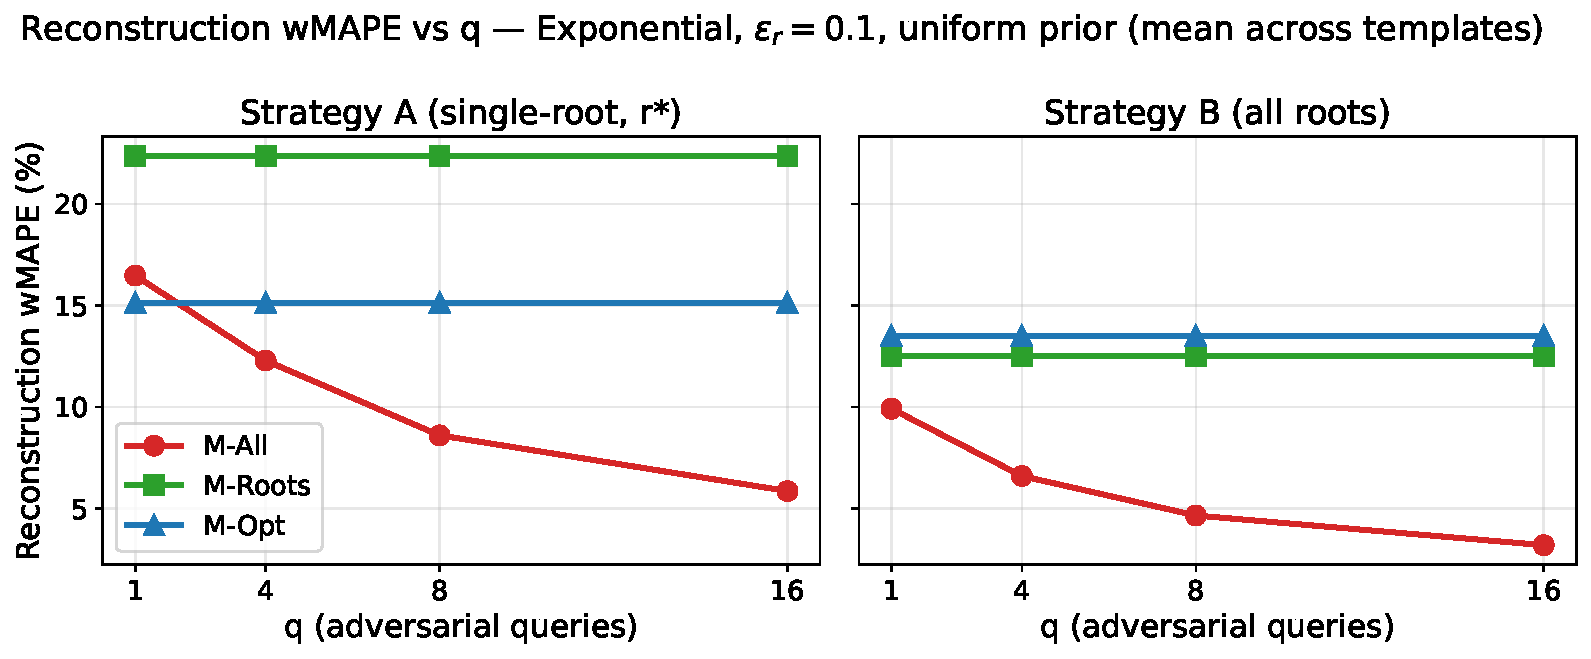
\includegraphics[width=\columnwidth]{figures/fig_mae_vs_q_eps0.1_uniform.pdf}
        \caption{Uniform prior. At $q = 1$, $\mathcal{M}$-All has $q+1 = 2$ observations on the targeted root, while $\mathcal{M}$-Roots has the cached value replayed twice. The gap at $q = 1$ reflects the second independent draw under $\mathcal{M}$-All; the divergence at $q > 1$ is the noise-averaging effect on accumulating draws.}
        \label{fig:recon_uniform}
    \end{subfigure}
    \begin{subfigure}[t]{\columnwidth}
        \centering
        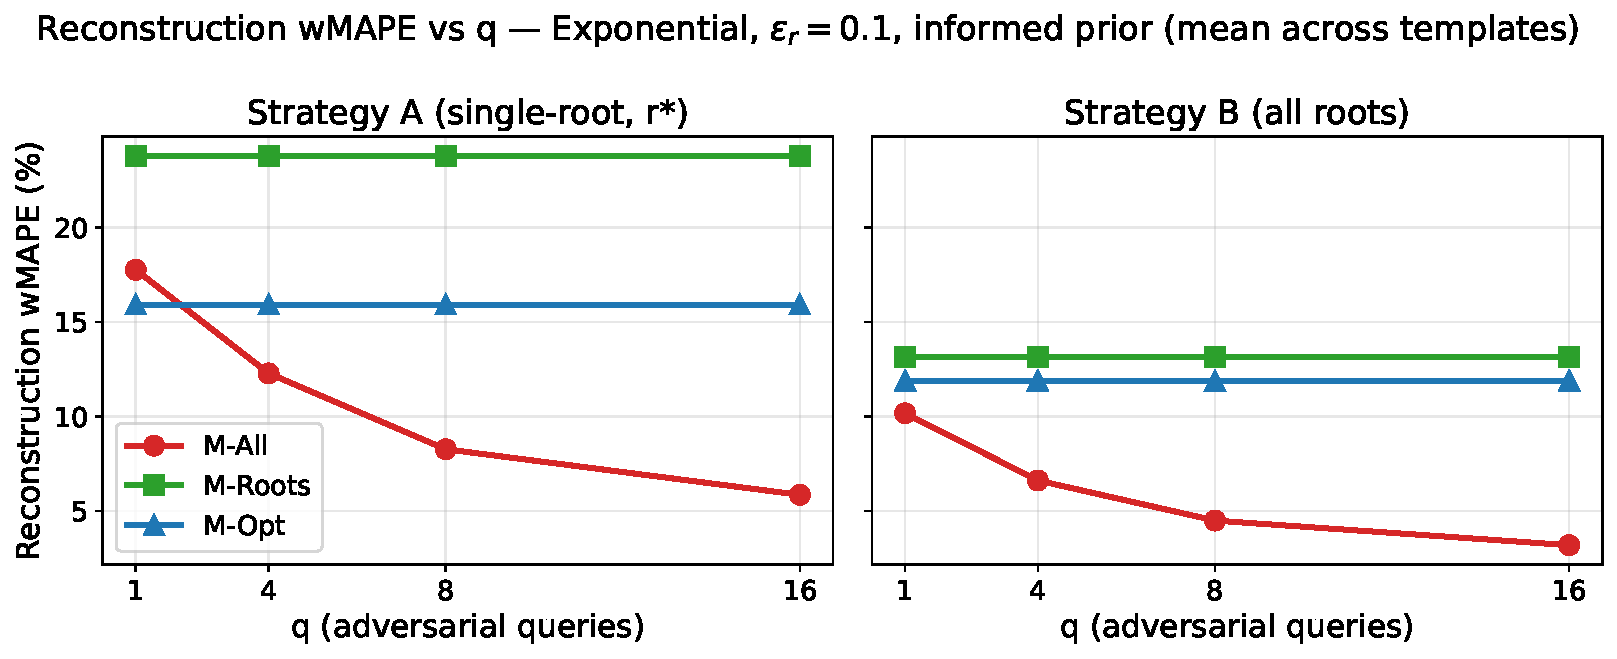
\includegraphics[width=\columnwidth]{figures/fig_mae_vs_q_eps0.1_informed.pdf}
        \caption{Informed prior. With Gaussian priors over unqueried roots, the qualitative behavior is unchanged from the uniform case: $\mathcal{M}$-All decreases monotonically with $q$; cached methods are flat.}
        \label{fig:recon_informed}
    \end{subfigure}
    \caption{Reconstruction wMAPE (\%) vs.\ adversarial query count $q$ at $\varepsilon_r = 0.1$ (Exponential, mean across 8 templates). Each row shows two strategies (A: single-root, B: all-roots). $\mathcal{M}$-All (red) degrades with $q$ in all settings; $\mathcal{M}$-Roots (green) and $\mathcal{M}$-Opt (blue) are flat.}
    \label{fig:recon_main}
\end{figure*}

\begin{table}[t]
\centering
\setlength{\tabcolsep}{2.5pt}
\small
\caption{Aggregate reconstruction wMAPE (\%) across privacy levels (Exponential, Strategy B, informed prior, mean across 8 templates). $\mathcal{M}$-All decreases with $q$ at every $\varepsilon_r$; $\mathcal{M}$-Roots and $\mathcal{M}$-Opt are invariant. Lower values mean the adversary reconstructs more accurately (worse for privacy).}
\label{tab:recon_main}
\begin{tabular}{c|ccc|ccc|ccc|ccc}
\toprule
& \multicolumn{3}{c|}{$q=1$} & \multicolumn{3}{c|}{$q=4$} & \multicolumn{3}{c|}{$q=8$} & \multicolumn{3}{c}{$q=16$} \\
$\varepsilon_r$ & All & Rts & Opt & All & Rts & Opt & All & Rts & Opt & All & Rts & Opt \\
\midrule
0.05 & 16.4 & 22.8 & 21.0 & 10.9 & 22.8 & 21.0 & 8.6  & 22.8 & 21.0 & 6.4 & 22.8 & 21.0 \\
0.1  & 10.2 & 13.2 & 11.9 & 6.6  & 13.2 & 11.9 & 4.5  & 13.2 & 11.9 & 3.2 & 13.2 & 11.9 \\
0.5  & 2.8  & 2.9  & 3.4  & 1.3  & 2.9  & 3.4  & 0.9  & 2.9  & 3.4  & 0.6 & 2.9  & 3.4 \\
1.0  & 1.4  & 1.5  & 2.3  & 0.7  & 1.5  & 2.3  & 0.5  & 1.5  & 2.3  & 0.3 & 1.5  & 2.3 \\
\bottomrule
\end{tabular}
\end{table}

\paragraph{Source of leakage.}
The result reveals a single effect compromising $\mathcal{M}$-All's privacy: \emph{repeated query accumulation}. Each adversarial query produces a fresh independent observation on the queried root, and the target turn contributes one additional fresh draw under $\mathcal{M}$-All (replayed cached value under \sysname{}). As $q$ grows, the adversary accumulates $q+1$ independent observations on each affected root and combines them via per-root MAP, tightening the posterior around the true value. The reduction in MAE follows the standard $1/\sqrt{q+1}$ scaling for averaged estimators of a fixed parameter under additive noise. \sysname{}'s cached methods provide no additional information after the first observation: every subsequent query returns the same value, leaving the per-root MAP unchanged.

\paragraph{Strategy A}
Fig.~\ref{fig:recon_uniform} (left panel) shows the targeted-root reconstruction. At $q = 1$, $\mathcal{M}$-All has 2 observations on $r^*$ (one query plus the target turn) while $\mathcal{M}$-Roots has the cached value replayed twice; the gap (16.5\% vs.\ 22.4\% aggregate) is purely the gain from a second independent draw under $\mathcal{M}$-All. As $q$ grows, $\mathcal{M}$-All's MAE drops to 12.3\% ($q = 4$), 8.6\% ($q = 8$), and 5.9\% ($q = 16$), tracking the expected $1/\sqrt{q+1}$ noise-averaging rate. $\mathcal{M}$-Roots and $\mathcal{M}$-Opt remain flat: at every $q$, $\mathcal{M}$-Roots reconstructs $r^*$ with 22.4\% wMAPE (the per-root error of one $\varepsilon_r$-noised release), and $\mathcal{M}$-Opt achieves 15.1\% because it concentrates budget on $r^*$ ($\varepsilon_{r^*} > \varepsilon_r$). The $2.8\times$ reduction ($16.5\% \to 5.9\%$) under $\mathcal{M}$-All is entirely attributable to independent noise averaging.

The informed prior (Fig.~\ref{fig:recon_informed}, left panel) gives nearly identical results because the target release does not enter the MAP --- the only effect of the informed prior on the targeted root is a soft regularization toward the population mean. At $\varepsilon_r = 0.1$: $\mathcal{M}$-All starts at 17.8\% (vs.\ 16.5\% uniform), drops to 5.9\% at $q = 16$. $\mathcal{M}$-Roots remains at 23.8\%. The qualitative result is unchanged.

\paragraph{Strategy B}
Table~\ref{tab:recon_main} shows that the pattern is consistent across all privacy levels. At $\varepsilon_r = 0.05$ (strong privacy), $\mathcal{M}$-All drops from $16.4\%$ to $6.4\%$ as $q$ goes from $1$ to $16$, while $\mathcal{M}$-Roots and $\mathcal{M}$-Opt remain at $22.8\%$ and $21.0\%$ respectively. At $\varepsilon_r = 0.1$, $\mathcal{M}$-All drops from $10.2\%$ to $3.2\%$ ($3.2\times$ reduction), against flat cached methods at $13.2\%$ ($\mathcal{M}$-Roots) and $11.9\%$ ($\mathcal{M}$-Opt). At $\varepsilon_r = 0.5$ (moderate privacy), $\mathcal{M}$-All drops from $2.8\%$ to $0.6\%$, while $\mathcal{M}$-Roots stays at $2.9\%$. At $q = 16$, $\mathcal{M}$-All reconstructs $4$--$5\times$ more accurately than $\mathcal{M}$-Roots across every privacy level. The per-template breakdown (Table~\ref{tab:rq2_per_template}, App.~\ref{app:rq2-tables}) confirms $\mathcal{M}$-All degrades on every template, with the largest absolute degradation on templates with wide root domains (HOMA: $19.1\% \to 5.1\%$, NLR: $20.9\% \to 7.6\%$ at $\varepsilon_r = 0.1$, informed prior).

% \begin{figure*}[t]
%     \centering
%     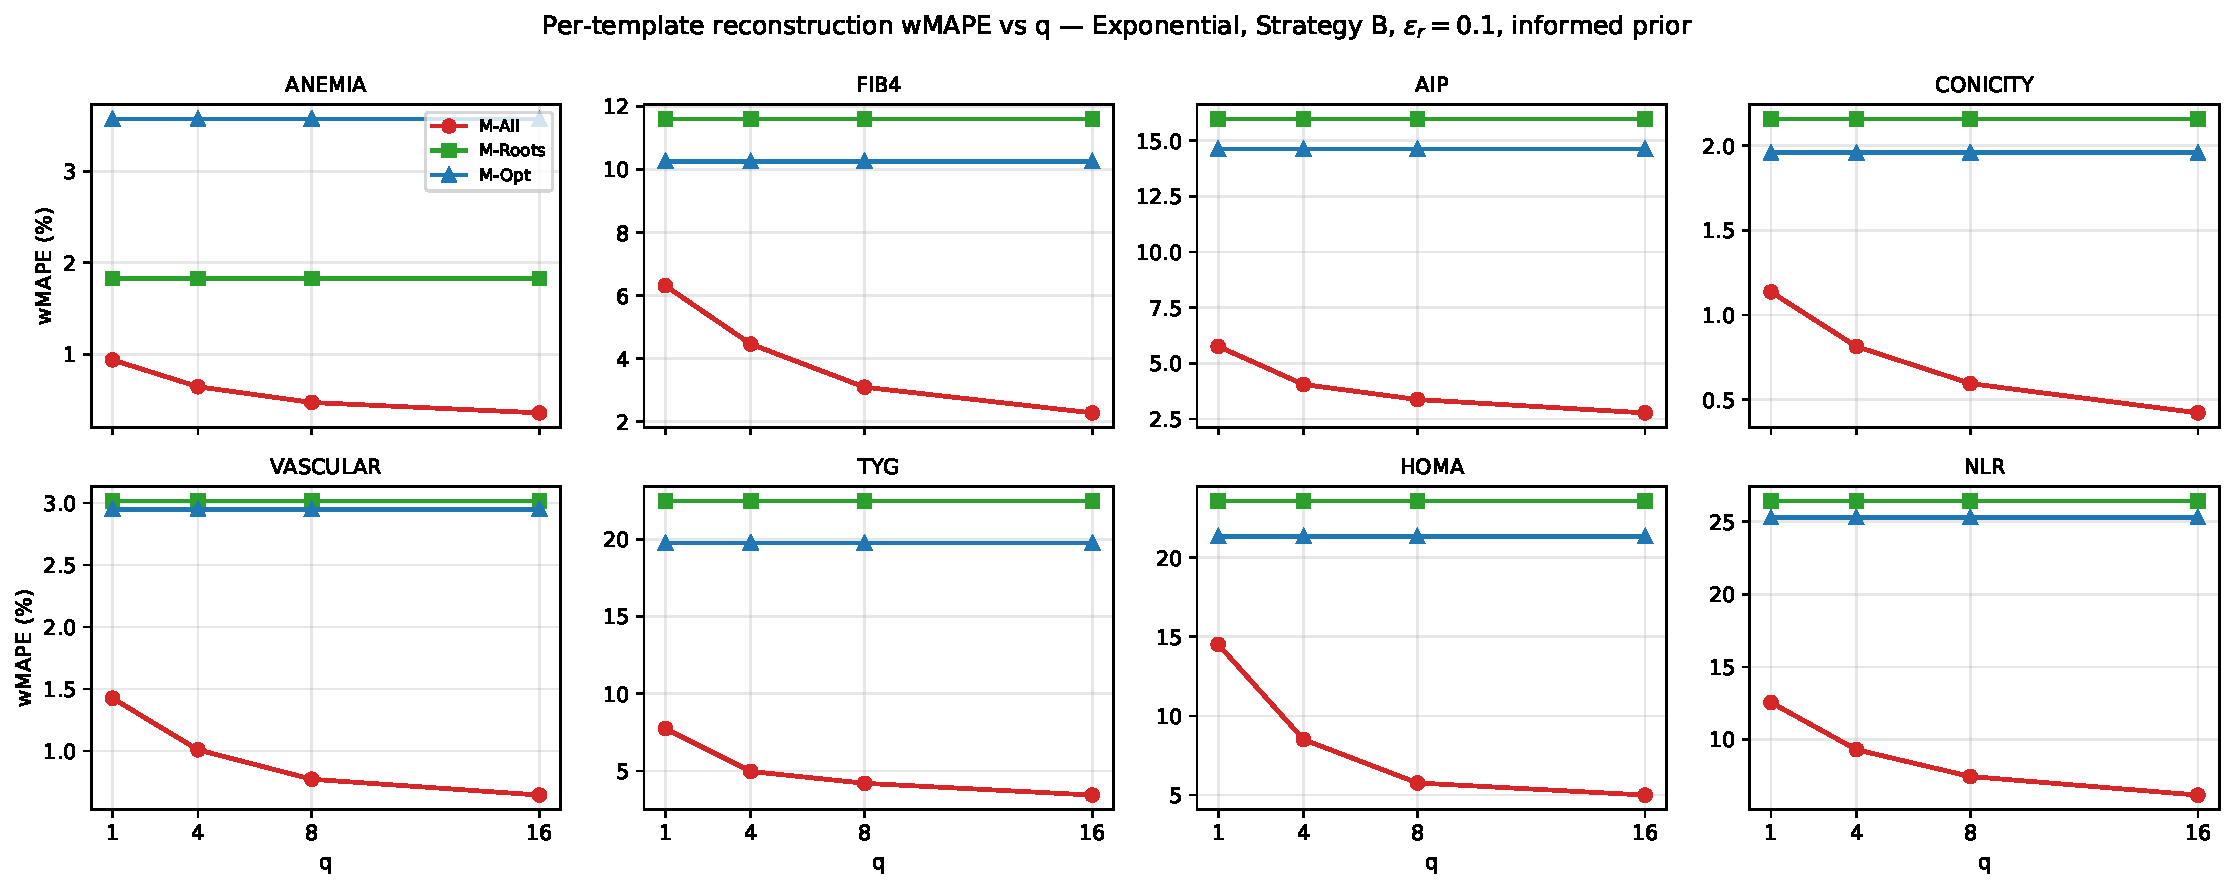
\includegraphics[width=\linewidth]{figures/grid_exp_B_eps0.1_informed.pdf}
%     \caption{Per-template reconstruction wMAPE (\%) vs.\ $q$ at $\varepsilon_r = 0.1$ (Exponential, Strategy B, informed prior). $\mathcal{M}$-All degrades on every template; $\mathcal{M}$-Roots and $\mathcal{M}$-Opt are flat.}
%     \label{fig:recon_per_template}
% \end{figure*}

\paragraph{$\mathcal{M}$-Opt vs.\ $\mathcal{M}$-Roots.}
The two cached methods show complementary behavior across strategies. In Strategy A, $\mathcal{M}$-Opt achieves lower MAE than $\mathcal{M}$-Roots on the targeted root ($15.1\%$ vs.\ $22.4\%$ aggregate, uniform prior) because it concentrates budget on $r^*$. In Strategy B, $\mathcal{M}$-Roots sometimes achieves lower \emph{average} MAE than $\mathcal{M}$-Opt --- for example, ANEMIA: M-Roots $1.9\%$ vs.\ M-Opt $3.6\%$ --- because $\mathcal{M}$-Opt starves low-sensitivity roots (e.g., RBC at $\varepsilon_{\min}$), making them harder to reconstruct, which increases the average. This illustrates a tradeoff: $\mathcal{M}$-Opt protects the most sensitive root but at the cost of higher average reconstruction error across all roots.

\paragraph{Key result}
$\mathcal{M}$-All's reconstruction MAE decreases monotonically with $q$ at every privacy level, every template, and under both priors. $\mathcal{M}$-Roots and $\mathcal{M}$-Opt are invariant to $q$. Under a worst-case adversary, $\mathcal{M}$-All's privacy degrades with each additional query; \sysname{} maintains a constant guarantee determined solely by the initial root noising. The Bounded Laplace and Staircase mechanisms exhibit the same pattern (App.~\ref{app:rq2-tables}).

Our reconstruction experiments use direct root queries, which is the simplest adversary strategy. Under $\mathcal{M}$-All, nonlinear derived-function queries could further amplify the adversary's advantage (Sec.~\ref{sec:nonlinear-amplification}); exploring optimal adversary function choice is left to future work. Under \sysname{}, function choice is irrelevant by Theorem~\ref{thm:privacy-guarantee}. Our results are therefore conservative estimates of $\mathcal{M}$-All's vulnerability.





\subsection{RQ3: Structural Analysis}
\label{sec:experiments-rq3}
\input{figures/rq4_aggregate_wmape}


RQ1 showed that $\mathcal{M}$-Opt consistently outperforms $\mathcal{M}$-Roots in aggregate, demonstrating that \emph{how} the budget is distributed matters beyond eliminating redundant noising. We now examine the structural conditions that determine the magnitude of \sysname{}'s advantage and the allocation properties that drive it. \sysname{} wins on every (template, mechanism, $\varepsilon$) cell at $B = (2k{+}1)\varepsilon$ and above; the size of the gap, however, varies substantially across templates, tracking two structural factors: (1) whether the target formula compresses or amplifies root noise, and (2) the geometry of the sensitivity-weighted budget allocation across roots. Per-template win counts across all mechanisms and privacy levels are reported in App.~\ref{app:rq3-winrate} (Table~\ref{tab:rq1_win_rate}).

% ────────────────────────────────────────────────────────────────────────
\subsubsection{Per-template analysis.}
\label{sec:per-template}

All per-template numbers in this section are reported at $B = (2k{+}1)\varepsilon$ for the Exponential mechanism unless otherwise noted. Full per-template wMAPE curves across $\varepsilon$ and all three mechanisms are in App.~\ref{app:rq1-tables-figs} (Fig.~\ref{fig:per_template_app}).

The per-template breakdown sorts templates into two regimes (Table~\ref{tab:per_template_summary}). \emph{Compressing} target formulas (logarithms, divisions by large constants) attenuate root noise into a wide target domain, leaving large headroom for $\mathcal{M}$-All to err and for \sysname{} to recover utility (AIP, HOMA, FIB4, NLR; absolute gaps $14$--$29$\,pp). \emph{Amplifying} formulas project root noise into narrow target domains, producing small absolute errors for both methods but preserving a $2$--$3\times$ multiplicative advantage for \sysname{} (ANEMIA, CONICITY, TYG, VASCULAR; gaps $\leq 4$\,pp). Across all 8 templates, no template falls below $2.1\times$ at $B = (2k{+}1)\varepsilon$; the pattern holds across all three mechanisms (App.~\ref{app:rq1-tables}) and grows more pronounced at $(3k{+}1)\varepsilon$, where ratios reach $3.0$--$5.4\times$.

\begin{table}[h]
\centering
\setlength{\tabcolsep}{4pt}
\small
\caption{Per-template wMAPE (\%) at $\varepsilon = 0.1$, $B = (2k{+}1)\varepsilon$ (Exponential). \emph{Compressing} formulas show large absolute gaps; \emph{amplifying} formulas show small absolute gaps but comparable multiplicative ratios. Full per-template tables in App.~\ref{app:rq1-tables}.}
\label{tab:per_template_summary}
\begin{tabular}{l l c c c}
\toprule
\textbf{Template} & \textbf{Formula} & \textbf{All} & \textbf{Opt} & \textbf{Ratio} \\
\midrule
\multicolumn{5}{l}{\emph{Compressing — large absolute gaps}} \\
AIP   & $\log_{10}(\text{TG}/\text{HDL})$           & 41.9 & 12.7 & $3.3\times$ \\
HOMA  & $\text{Glu}\cdot\text{Ins}/405$              & 31.1 &  9.9 & $3.1\times$ \\
NLR   & $\text{NEU}/\text{LYM}$                      & 49.2 & 23.1 & $2.1\times$ \\
FIB4  & $\text{age}\cdot\text{AST}/(\text{PLT}\sqrt{\text{ALT}})$ & 23.9 & 10.0 & $2.4\times$ \\
\midrule
\multicolumn{5}{l}{\emph{Amplifying — small absolute gaps}} \\
VASCULAR & $100(\text{SBP}{-}\text{DBP})/\text{SBP}$ &  6.3 &  2.6 & $2.4\times$ \\
TYG      & $\ln(\text{TG}\cdot\text{Glu}/2)$         &  4.6 &  2.0 & $2.3\times$ \\
CONICITY & $\text{waist}/(0.109\sqrt{\text{wt}/\text{ht}})$ &  2.8 &  1.0 & $2.8\times$ \\
ANEMIA   & $100\cdot\text{Hb}/\text{Hct}$            &  2.4 &  0.7 & $3.3\times$ \\
\bottomrule
\end{tabular}
\end{table}

\subsubsection{Power-law allocation and mechanism independence.}

The closed-form approximation (Sec.~\ref{sec:opt-budget}) predicts $\varepsilon_i \propto (|h_i| \cdot D_i)^{1/2}$. Empirically, normalized per-root allocations across all 8 templates collapse onto a single log-log line with fitted slope 0.50 (Exponential, $\varepsilon = 0.1$, $B = (2k{+}1)\varepsilon$; full plot in App.~\ref{app:per-root-budget}, Fig.~\ref{fig:allocation_powerlaw_app}), confirming the prediction. Roots with higher sensitivity--domain products receive proportionally more budget.

% The closed-form approximation (Sec.~\ref{sec:opt-budget}) predicts $\varepsilon_i \propto (|h_i| \cdot D_i)^{1/2}$. Fig.~\ref{fig:allocation_powerlaw} verifies this empirically: on a log-log scale, the normalized per-root allocations across all 8 templates collapse onto a single line with fitted slope 0.50 (Exponential, $B = (2k{+}1)\varepsilon$, $\varepsilon = 0.1$). Roots with higher sensitivity--domain products, which contribute more to the target value, receive proportionally more budget.

The allocation is mechanism-independent: at $\varepsilon = 0.1$, all three mechanisms produce fitted slopes of exactly 0.50; at $\varepsilon = 0.5$, minor deviations appear (Exp 0.49, BLap 0.52, Stair 0.51). Full three-mechanism plots at all privacy levels are in App.~\ref{app:per-root-budget}. This confirms that the budget distribution is governed by the DAG's sensitivity geometry, not the noise distribution. A deployment can switch mechanisms without recomputing the allocation.

% \begin{figure}[t]
%     \centering
%     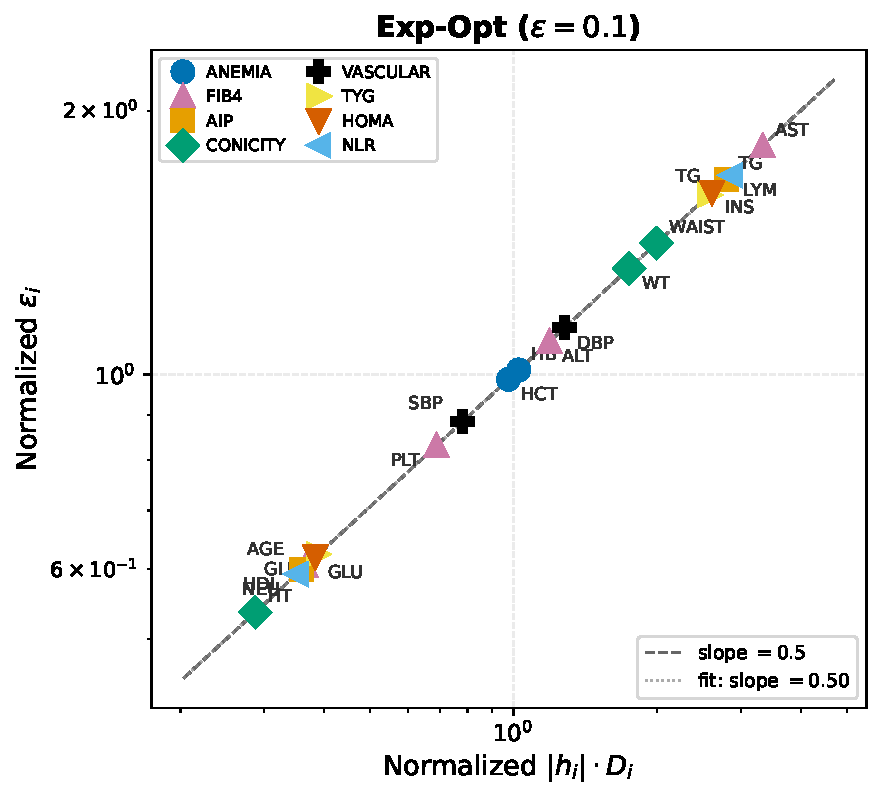
\includegraphics[width=\columnwidth]{figures/rq2_allocation_powerlaw_2kplus1_Exp_eps0p1.pdf}
%     \caption{Log-log scatter of normalized per-root budget $\varepsilon_i$ vs.\ sensitivity--domain product $|h_i| \cdot D_i$ (Exponential, $\varepsilon = 0.1$, $B = (2k{+}1)\varepsilon$). All 8 templates, active roots only. Fitted slope = 0.50. Roots are labeled by medical attribute.}
%     \label{fig:allocation_powerlaw}
% \end{figure}

\subsubsection{Zero-sensitivity roots.}

Some roots have zero sensitivity to the target: RBC in ANEMIA ($\partial \text{MCHC}/\partial \text{RBC} = 0$) and TC in AIP ($\partial \text{AIP}/\partial \text{TC} = 0$). Under $\mathcal{M}$-Roots, these consume $1/k$ of the budget without reducing target error. Under $\mathcal{M}$-Opt, they are clamped at $\varepsilon_{\min}$ and their share is redistributed, effectively giving each active root $50\%$ more budget on these 3-root templates.

This creates complementary effects in the two RQs. In RQ1, the budget reclamation amplifies \sysname{}'s advantage on these 3-root templates: each active root receives effectively $50\%$ more budget than under uniform allocation, contributing to the strong multiplicative wins on ANEMIA ($3.3\times$) and AIP ($3.3\times$) at $\varepsilon = 0.1$, $B = (2k{+}1)\varepsilon$. In RQ2, the clamped roots are very hard to reconstruct (high noise), increasing $\mathcal{M}$-Opt's average reconstruction MAE under Strategy B (e.g., ANEMIA: M-Opt $3.6\%$ vs.\ M-Roots $1.9\%$) --- while simultaneously making the high-budget roots harder for an adversary to improve upon under Strategy A.

%%%%%%%%%%%%%%%%%%%%%%%%%%%%%%%%%%%%%%%%%%%%%%%%%%%%%
%%%%%%%%%%%%%%%%%%%%%%%%%%%%%%%%%%%%%%%%%%%%%%%%%%%%%
%%%%%%%%%%%%%%%%%%%%%%%%%%%%%%%%%%%%%%%%%%%%%%%%%%%%%
\subsection{RQ4: End-to-End Deployment in an LLM Tool-Call Pipeline}
\label{sec:experiments-rq4}

RQ1--3 establish the privacy-utility tradeoff at the mechanism level, with the user agent and adversary simulated directly through mechanism implementations. We now ask: do these findings transfer to a real LLM-driven tool-call deployment, where the user agent is an LLM that parses natural-language queries, sanitizes via the mechanism, and emits structured replies through a tool-call interface?

\subsubsection{Setup.}
We instantiate the user agent with GPT-5.4 nano, configured as a tool-using assistant that holds the patient's private root values and responds to per-turn queries from an adversarial service. Each session implements the same threat model as RQ1 (Sec.~\ref{sec:threat-model}): the adversary requests root values or derived computations across $t \in \{k{+}1, 2k{+}1, 3k{+}1\}$ turns, with the final turn requesting all roots required to compute the target. The sanitization mechanism is the discrete Exponential under each of the three configurations ($\mathcal{M}$-All, $\mathcal{M}$-Roots, $\mathcal{M}$-Opt). All values cross the trust boundary as natural-language responses parsed by the adversary via an alias-resolving regex parser (App.~\ref{app:agent-eval}). Per-cell budget allocations for $\mathcal{M}$-Roots and $\mathcal{M}$-Opt are fixed in advance (population-mean sensitivities) and shared with the user agent at session initialization.

\paragraph{Scale.} We sweep 8 templates $\times$ 3 configurations $\times$ 3 turn budgets $\times$ 3 privacy levels ($\varepsilon \in \{0.01, 0.05, 0.1\}$) with 100 patients per cell, for a total of \textbf{21{,}600 sessions} and \textbf{161{,}784 sanitized observations}. All patients are drawn deterministically from the NHANES holdout (the same 100-patient subsets used in RQ1).

\subsubsection{Aggregate ordering reproduces.}
Table~\ref{tab:agent_aggregate_wmape} reports aggregate wMAPE across the agent-eval sweep. The ordering $\mathcal{M}$-All $>$ $\mathcal{M}$-Roots $>$ $\mathcal{M}$-Opt holds at every cell, matching RQ1. At $\varepsilon = 0.1$, $B = (2k{+}1)\varepsilon$, agent-eval $\mathcal{M}$-Opt achieves $7.6\% \pm 0.5\%$ vs.\ $\mathcal{M}$-All's $22.2\% \pm 1.2\%$ --- a $2.9\times$ improvement, agreeing with RQ1's $2.6\times$ ($7.8\%$ vs.\ $20.3\%$) within $0.12$pp at the focal cell and within $\pm 1.9$pp across all nine $(\varepsilon, B)$ aggregate cells.

% Table~\ref{tab:agent_aggregate_wmape} reports aggregate wMAPE across the agent-eval sweep. The ordering $\mathcal{M}$-All $>$ $\mathcal{M}$-Roots $>$ $\mathcal{M}$-Opt holds at every cell, matching RQ1. At $\varepsilon = 0.1$, $B = (2k{+}1)\varepsilon$, agent-eval $\mathcal{M}$-Opt achieves $7.6\% \pm 0.5\%$ vs.\ $\mathcal{M}$-All's $22.2\% \pm 1.2\%$ --- a $2.9\times$ improvement, indistinguishable from RQ1's $2.6\times$ ($7.8\%$ vs.\ $20.3\%$) within bootstrap noise.

\subsubsection{Per-template structure reproduces.}
The per-template ordering matches RQ1's structural analysis (Sec.~\ref{sec:experiments-rq3}). Templates with compressing target formulas (AIP, HOMA, FIB4) yield the largest absolute gaps under deployment as in the controlled harness; templates with amplifying formulas (ANEMIA, CONICITY) yield smaller absolute gaps. $\mathcal{M}$-Opt strictly improves on $\mathcal{M}$-All in $9/9$ (B, $\varepsilon$) cells for 7 of 8 templates; the eighth (NLR) shows $\mathcal{M}$-Opt $<$ $\mathcal{M}$-All in $7/9$ cells, reflecting NLR's narrow target domain and high baseline noise variance, where bootstrap intervals on M-All and M-Opt overlap at $B = (k{+}1)\varepsilon$.

\subsubsection{Pipeline robustness.}
The deployment-layer integration is end-to-end clean. Across 21{,}600 sessions and 161{,}784 sanitized observations we observed \textbf{zero}:
\begin{itemize}
    \item sessions with parse failures (the LLM never emitted a malformed response that broke the adversary's parser).
    \item observation-level parse failures.
    \item NaN target outputs (every session produced a numeric target the adversary could consume).
    \item rounding gaps between the LLM's text reply and the underlying mechanism's wire-format output.
\end{itemize}

\noindent The combination of zero compliance failures and quantitative agreement with RQ1 confirms that the dependency-aware sanitization layer survives a real tool-call pipeline without leaking utility or privacy through implementation friction.

% \subsubsection{Cross-validation against RQ1.}
% At $\varepsilon = 0.1$, the agent-eval and RQ1 wMAPE values agree within $\pm 1.9$pp absolute across all nine $(\varepsilon, B)$ aggregate cells, with the headline cell ($\varepsilon = 0.1$, $B = (2k{+}1)\varepsilon$, $\mathcal{M}$-Opt) agreeing within $0.12$pp ($7.64\%$ deployment vs.\ $7.76\%$ harness). At lower $\varepsilon$ ($0.01$), where wMAPE is already saturated above $80\%$, absolute pp gaps grow but the qualitative ordering and per-template structure hold. This level of agreement is expected --- the two evaluations share patient data, mechanism, allocation, and threat model, differing only in the user-agent layer (LLM tool-call vs.\ direct mechanism call). The cross-validation confirms that LLM-side parsing, formatting, and prompt-handling do not introduce systematic biases at the operating points where the privacy-utility tradeoff is most informative.

\paragraph{Scope of evaluation.}
Our deployment evaluation covers the discrete Exponential mechanism only ($\mathcal{M}$-All, $\mathcal{M}$-Roots, $\mathcal{M}$-Opt) at three $\varepsilon$ levels and one LLM (GPT-5.4 nano). Bounded Laplace and Staircase mechanisms are evaluated in RQ1 but not re-run through the LLM harness; their RQ1 patterns are mechanism-agnostic at the allocation level (Sec.~\ref{sec:experiments-rq3}, mechanism-independent power law), giving us no reason to expect different deployment behavior, but a direct test would require additional sessions. We make no claims about other LLM backbones or harnesses; the result is that \emph{this} deployment configuration reproduces RQ1, not that all configurations will. Fully autonomous LLM deployments where the user agent reasons about which values to disclose --- rather than executing a deterministic sanitization protocol --- are out of scope.